\noindent\textbf{Notation.}
Assume $f^0: \mathcal{X} \rightarrow \mathcal{Y}$ is a BB, trained on a dataset $\mathcal{X} \times\mathcal{Y} \times \mathcal{C}$, with $\mathcal{X}$, $\mathcal{Y}$, and $\mathcal{C}$ being the images, classes, and concepts, respectively; $f^0=h^0 \circ \Phi$, where $\Phi$ and  $h^0$ is the feature extractor and the classifier respectively. Also, $m$ is the number of class labels. This paper focuses on binary classification (having or not having a disease), so $m=2$ and $\mathcal{Y} \in \{0, 1\}$. Yet, it can be extended to multiclass problems easily. Given a learnable projection~\cite{ghosh2023route}, $t: \Phi \rightarrow \mathcal{C}$, our method learns three functions: (1) a set of selectors ($\pi: \mathcal{C}\rightarrow \{0, 1\}$) routing samples to an interpretable model or residual, (2) a set of interpretable models ($g: \mathcal{C} \rightarrow \mathcal{Y}$), and (3) the residuals. The interpretable models are called ``experts" since they specialize in a distinct subset of data defined by that iteration's coverage $\tau$ as shown in SelectiveNet~\cite{rabanser2022selective}. Fig.~\ref{fig:schematic} illustrates our method.

\begin{figure*}[t]
\begin{center}
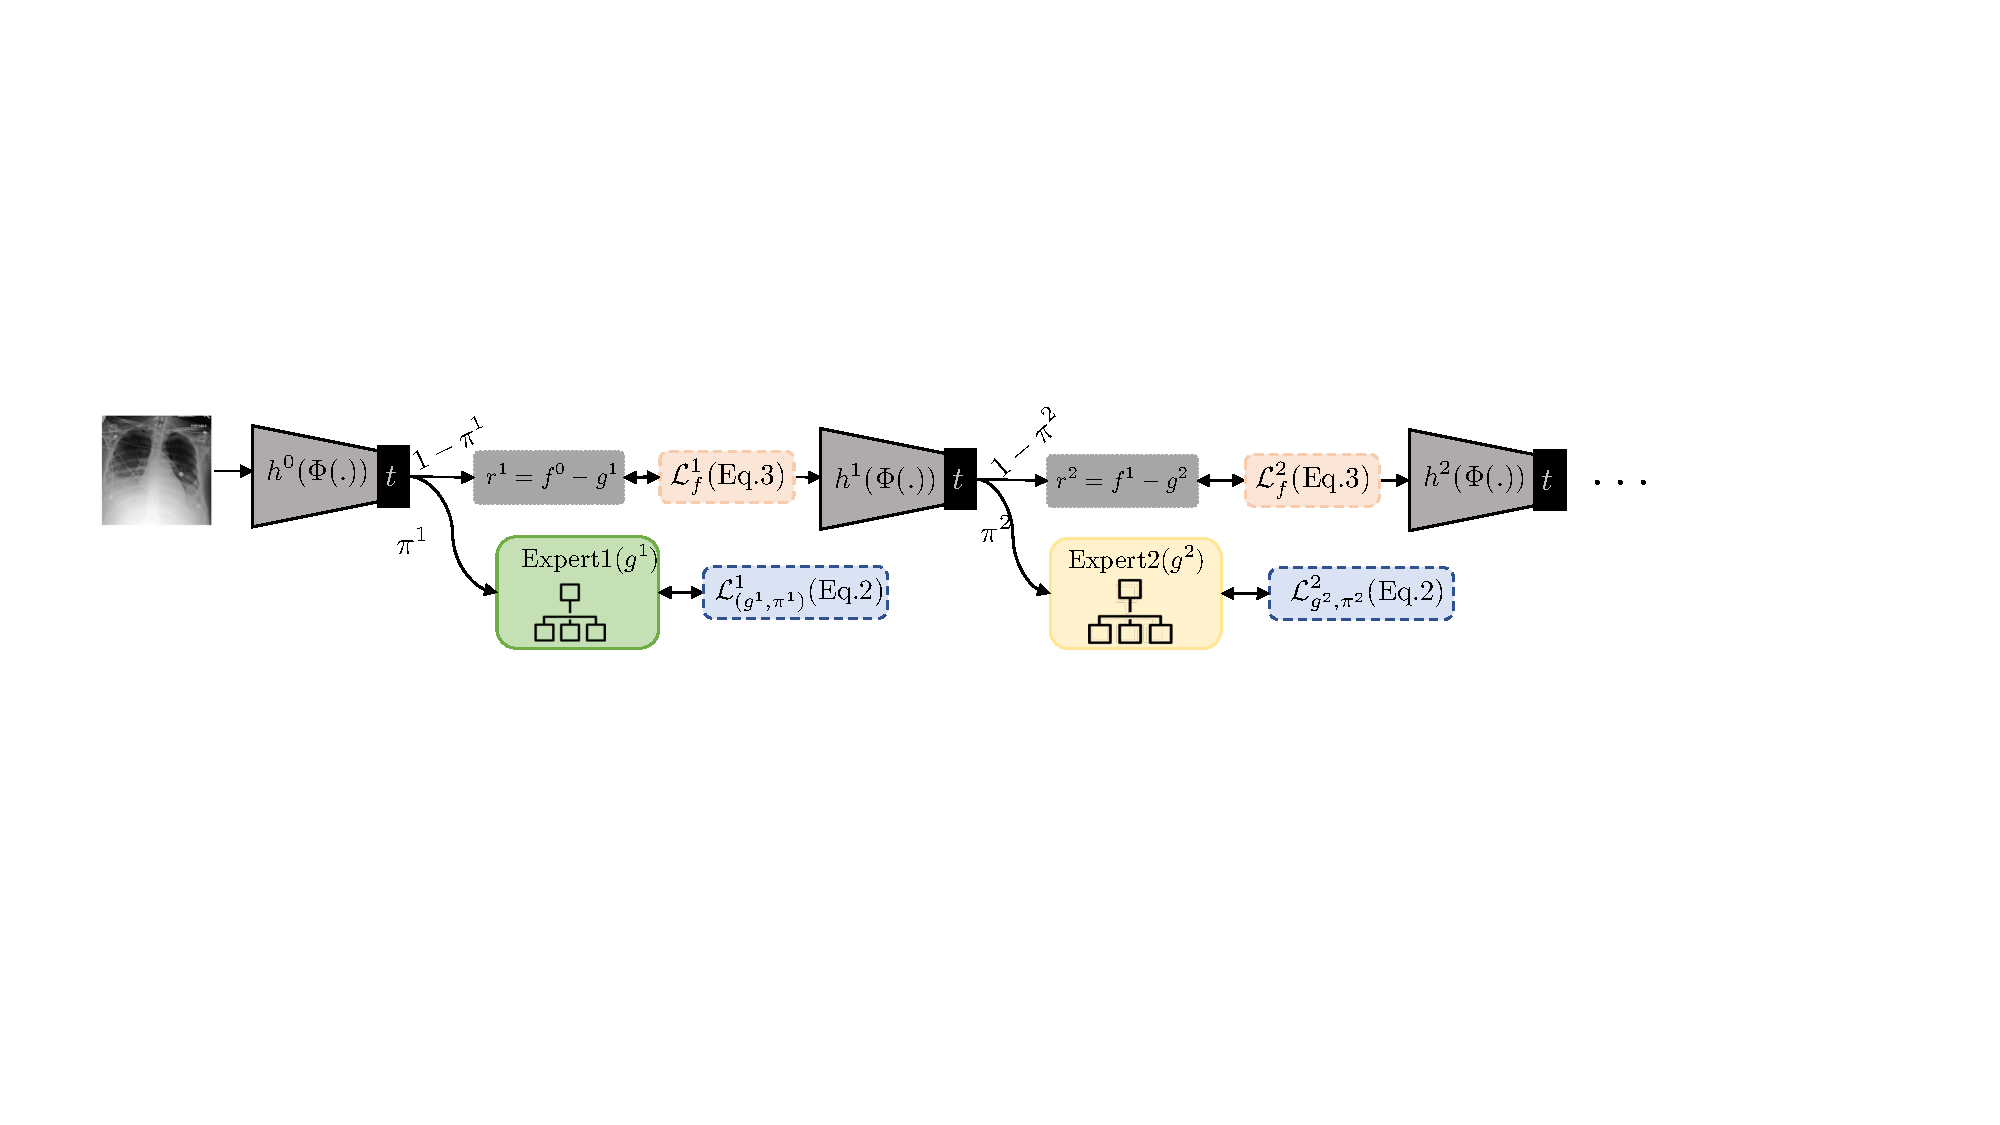
\includegraphics[width=\linewidth]{plots/main/Schematic.pdf}
\caption{Schematic view of our method. Note that $f^k(.) = h^k(\Phi(.))$. At iteration $k$, the selector \emph{routes} each sample either towards the expert $g^k$ with probability $\pi^k(.)$ or the residual $r^k = f^{k-1} - g^k$ with probability $1-\pi^k(.)$. $g^k$ generates FOL-based explanations for the samples it covers. Note $\Phi$ is fixed across iterations.}
\label{fig:schematic}
\end{center}
\end{figure*}

\subsection{Distilling BB to the mixture of interpretable models}
\noindent\textbf{Handling class imbalance.} For an iteration $k$, we first split the given coverage $\tau^k$ to stratified coverages per class as $\{\tau^k_m = w_m \cdot \tau^k; w_m=N_m/N, \forall m\}$, where $w_m$ denotes the fraction of samples belonging to the $m^{th}$ class; $N_m$ and $N$ are the samples of $m^{th}$ class and total samples, respectively. 
% The coverage is defined as the portion of data covered by all the interpretable models.
% With $\tau^k_m$, we modify the optimization strategy to learn the selectors and experts.

\noindent \textbf{Learning the selectors.}
At iteration $k$, the selector $\pi^k$ \emph{routes} $i^{th}$ sample to the expert ($g^k$) or residual ($r^k$) with probability $\displaystyle \pi^k(\boldsymbol{c_i})$ and $\displaystyle 1 - \pi^k(\boldsymbol{c_i})$ respectively. 
For coverages $\{\tau^k_m, \forall m\}$, we learn $g^k$ and $\pi^k$ jointly by solving the 
loss:
% following optimization problem:
\begin{align}
\label{equ: optimization_g}
\theta_{s^k}^*, \theta_{g^k}^* = & \operatorname*{arg\,min}_{\theta_{s^k}, \theta_{g^k}} \mathcal{R}^k\Big(\pi^k(.; \theta_{s^k}), \displaystyle g^k(.; \theta_{g^k}) \Big) 
~~\text{s.t.}~\zeta_m\big(\pi^k(.; \theta_{s^k})\big) \geq \tau^k_m ~~\forall m,
\end{align}
where $\theta_{s^k}^*, \theta_{g^k}^*$ are the optimal parameters for $\pi^k$ and $g^k$, respectively.
% $\mathcal{L}_{(g^k, \pi^k)}^k$ is the loss to distill BB ($f^{k-1}$) of the previous iteration $(k-1)$ to the current expert $g^k$ discussed following section. 
$\mathcal{R}^k$ is the overall selective risk, defined as,
% \begin{equation}
% \label{equ: emp_risk}
$\mathcal{R}^k(\displaystyle \pi^k, \displaystyle g^k) = \mathlarger{\sum}_m\frac{\frac{1}{N_m}\sum_{i=1}^{N_m}\mathcal{L}_{(g^k, \pi^k)}^k\big(\boldsymbol{x_i}, \boldsymbol{c_i}\big)}{\zeta_m(\pi^k)}$ ,
% \end{equation}
where $\zeta_m(\pi^k) = \frac{1}{N_m}\sum_{i=1}^{N_m}\pi^k(\boldsymbol{c_i})$ is the empirical mean of samples of $m^{th}$ class selected by the selector for the associated expert $\displaystyle g^k$. We define $\mathcal{L}_{(g^k, \pi^k)}^k$ in the next section.
The selectors are neural networks with sigmoid activation. At inference time, $\pi^k$ routes a sample  to $\displaystyle g^k$ if and only if $\pi^k(.)\geq 0.5$. 

\noindent \textbf{Learning the experts.}
\label{learn_explert}
For iteration $k$, the loss $\mathcal{L}_{(g^k, \pi^k)}^k$ distills the expert $g^k$ from $f^{k-1}$, BB of the previous iteration by solving the following loss:
\begin{equation}
\label{equ: g_k}
\resizebox{0.8\textwidth}{!}{$
\mathcal{L}_{(g^k, \pi^k)}^k\big(\boldsymbol{x_i}, \boldsymbol{c_i}\big) = \underbrace{\mystrut{2.6ex}\ell\Big(f^{k - 1}(\boldsymbol{x_i}), g^k(\boldsymbol{c_i})\Big)\pi^k(c_i) }_{\substack{\text{trainable component} \\ \text{for current iteration $k$}}}\underbrace{\prod_{j=1} ^{k - 1}\big(1 - \pi^j(\boldsymbol{c_i})\big)}_{\substack{\text{fixed component trained} \\ \text{in the previous iterations}}},
$}
\end{equation}
where $\pi^k(\boldsymbol{c_i})\prod_{j=1} ^{k - 1}\big(1 - \pi^j(\boldsymbol{c_i}) \big)$ is the cumulative probability of the sample covered by the residuals for all the previous iterations from $1, \cdots, k-1$ (\ie $\prod_{j=1} ^{k - 1}\big(1 - \pi^j(\boldsymbol{c_i}) \big)$\big) and the expert $g^k$ at iteration $k$ \big(\ie $\pi^k(\boldsymbol{c_i})$\big). 
% In this work, each $g^k$ is an Entropy-based linear layer neural network (ELL)~\cite{barbiero2022entropy} as ~\cite{ghosh2023route} to create a FOL-based explanation for a sample.

\noindent \textbf{Learning the Residuals.}
After learning $g^k$, we calculate the residual as, $r^k (x_i, c_i) = f^{k-1}(x_i) - g^k(c_i)$ (difference of logits). We fix $\Phi$ and optimize the following loss to update $h^k$ to specialize on those samples not covered by $g^k$, effectively creating a new BB $f^k$ for the next iteration $(k+1)$:
\begin{equation}
\label{equ: residual}
\mathcal{L}_f^k(\boldsymbol{x_j}, \boldsymbol{c_j}) = \underbrace{\mystrut{2.6ex}\ell\big(r^k(\boldsymbol{x_j}, \boldsymbol{c_j}), f^k(\boldsymbol{x_j})\big)}_{\substack{\text{trainable component} \\ \text{for iteration $k$}}} \underbrace{\mystrut{2.6ex}\prod_{i=1} ^{k}\big(1 - \pi^i(\boldsymbol{c_j})\big)}_{\substack{\text{non-trainable component} \\ \text{for iteration $k$}}}
\end{equation}
 We refer to all the experts as the Mixture of Interpretable Experts (MoIE-CXR). We denote the models, including the final residual, as MoIE-CXR+R. Each expert in MoIE-CXR constructs sample-specific FOLs using the optimization strategy and algorithm discussed in~\cite{ghosh2023route}.

\iffalse
\begin{figure*}[t]
\begin{center}
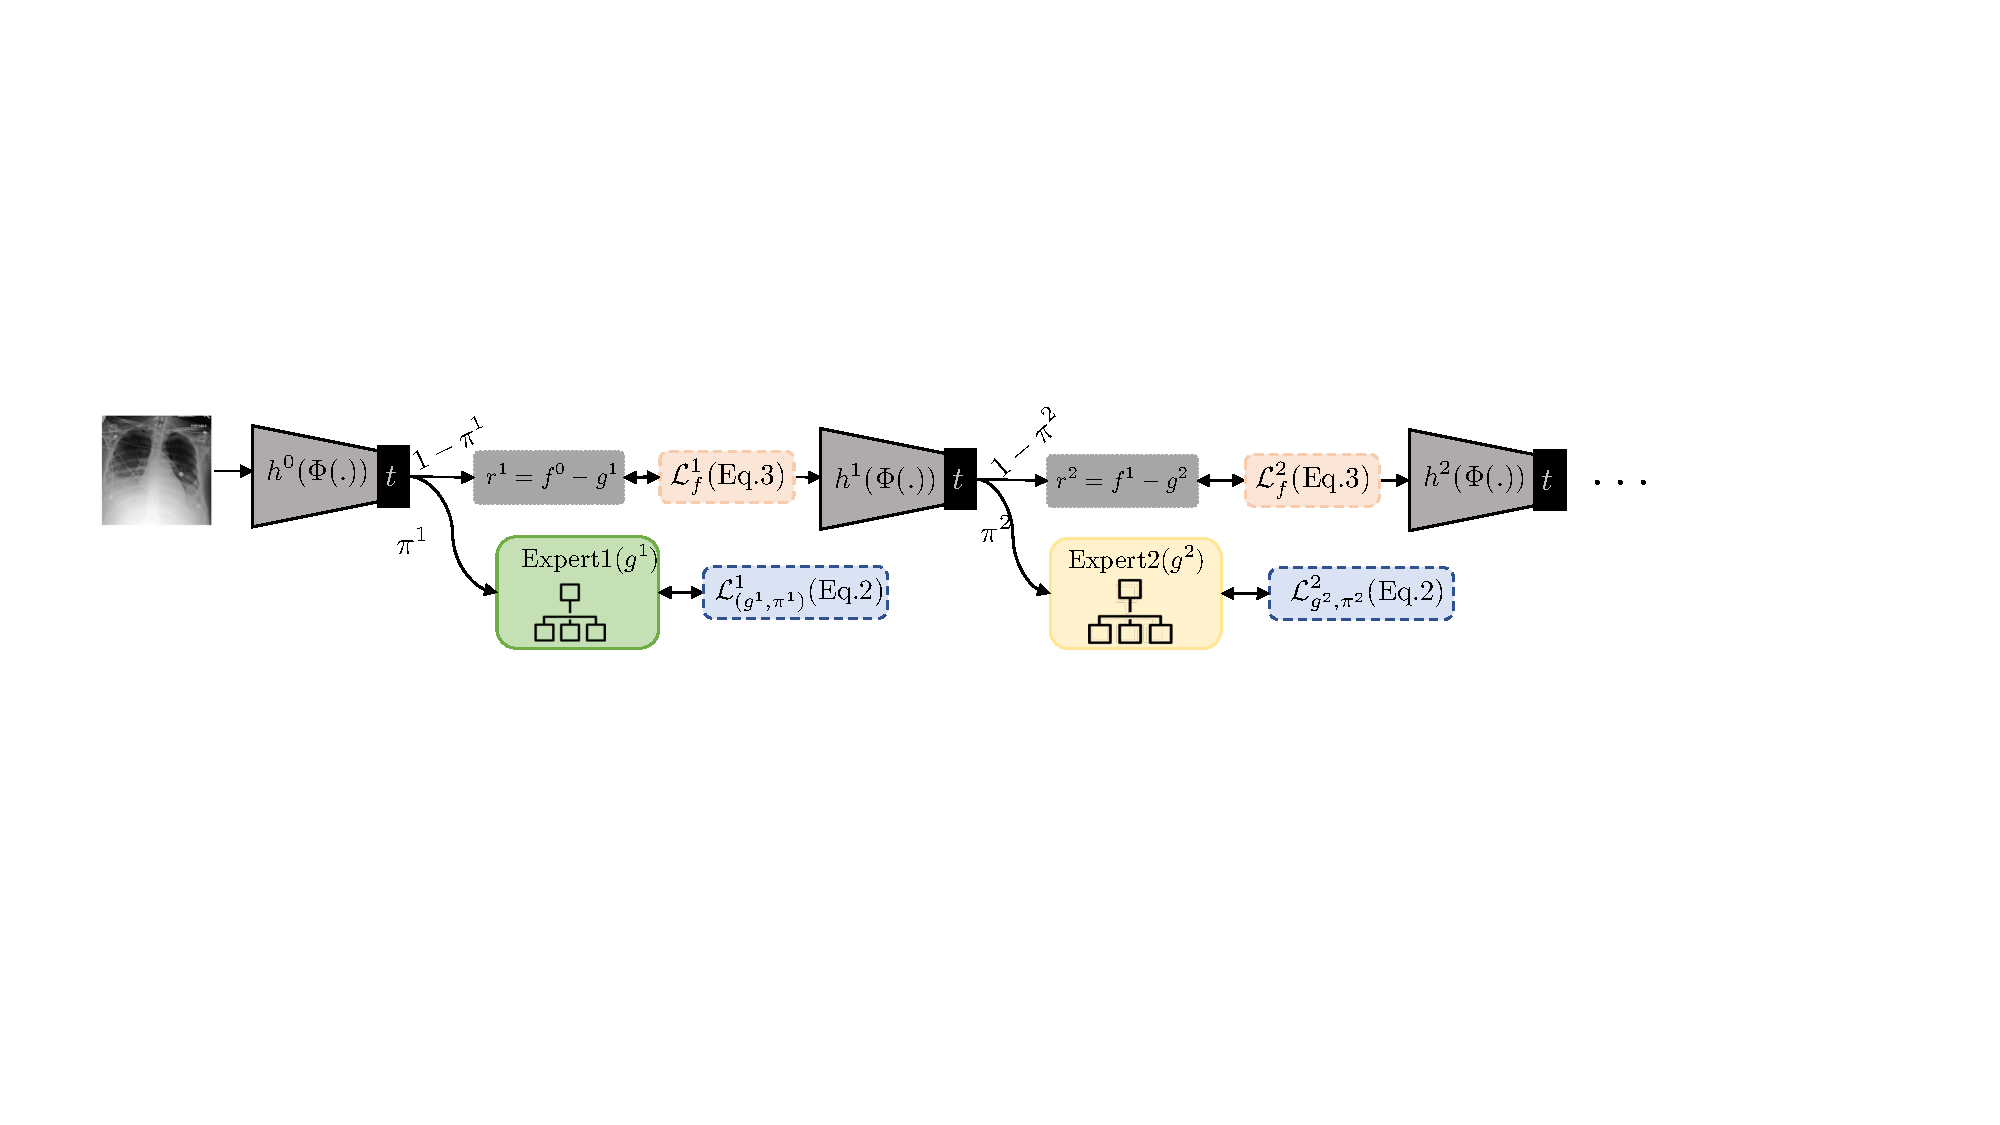
\includegraphics[width=\linewidth]{plots/main/Schematic.pdf}
\caption{Schematic view of our method. Note that $f^k(.) = h^k(\Phi(.))$. At iteration $k$, the selector \emph{routes} each sample either towards the expert $g^k$ with probability $\pi^k(.)$ or the residual $r^k = f^{k-1} - g^k$ with probability $1-\pi^k(.)$. $g^k$ generates FOL-based explanations for the samples it covers. Note $\Phi$ is fixed across iterations.}
\label{fig:schematic}
\end{center}
\end{figure*}
\fi

\subsection{Finetuning to an unseen domain} 
% The MoIE-CXR-identified concepts should be domain invariant. 
We assume the MoIE-CXR-identified concepts to be generalizable to an unseen domain. So, we learn the projection $t_t$ for the target domain and compute the pseudo concepts using SSL~\cite{lee2013pseudo}. Next, we transfer the selectors, experts, and final residual ($\{\pi^k_s, g^k_s\}_{k=1}^K$ and $f^K_s$) from the source to a target domain with limited labeled data and computational cost.
% First, we identify the correctly classified samples using the BB of the source domain ($f^0_s$) and compute the pseudo concepts for them using the projection of the source domain ($t_s$), keeping the misclassified samples as unlabelled. Next, we learn the projection $t_t$ of the target domain in semi-supervised fashion~\cite{lee2013pseudo} with the pseudo-labeled and unlabeled concepts. With $t_t$, we compute the concepts $\mathcal{C}_t$ for the target domain. Next using equations~\ref{equ: optimization_g},~\ref{equ: g_k} and~\ref{equ: residual}, we learn the $\{\pi^k_t, g^k_t\}_{k=1}^K$ and $f^K_t$ for the target domain.
Algorithm~\ref{algo: domain_transfer} details the procedure.

\begin{algorithm}[H]
   \caption{Finetuning to an unseen domain.}
   \label{algo: domain_transfer}
\begin{algorithmic}[1]
   \STATE {\bfseries Input:} Learned selectors, experts, and final residual from source domain: $\{\pi^k_s, g^k_s\}_{k=1}^K$ and $f^K_s$ respectively, with $K$ as the number of experts to transfer. BB of the source domain: $f_s^0=h^0_s(\Phi_s)$. Source data: $\mathcal{D}_s = \{\mathcal{X}_s, \mathcal{C}_s, \mathcal{Y}_s\}$. Target data: $\mathcal{D}_t = \{\mathcal{X}_t, \mathcal{Y}_t\}$. Target coverages $\{\tau_k\}_{k=1}^K$.
   \STATE {\bfseries Output:} Experts $\{\pi^k_t, g^k_t\}_{k=1}^K$ and final residual $f^K_t$ of the target domain.
   \STATE Randomly select $n_t\ll N_t$ samples out of $N_t=|\mathcal{D}_t|$.
   \STATE Compute the pseudo concepts for the correctly classified samples in the target domain using $f^0_s$, as, $\boldsymbol{c_t^i} = t_s\big(\Phi_s(\boldsymbol{x_s}^i)\big)$ \st $y_t^i=f^0_s(\boldsymbol{x_t}^i)$, $i=1 \cdots~n_t$
   \STATE \label{step:psudo-label} Learn the projection function $t_t$ for target domain semi-supervisedly~\cite{lee2013pseudo} using the pseudo labeled samples $\{\boldsymbol{x}_t^i, \boldsymbol{c}_t^i\}_{i=1}^{n_t}$ and unlabeled samples $\{\boldsymbol{x}_t^i\}_{i=1}^{N_t-n_t}$.
   \STATE Complete the triplet for the target domain \{$\mathcal{X}_t, \mathcal{C}_t, \mathcal{Y}_t$\}, where $\boldsymbol{c}_t^i=t_t(\Phi_s(\boldsymbol{x}_t^i))$, $i=1\cdots~N_t$.
   \STATE Finetune $\{\pi^k_s, g^k_s\}_{k=1}^K$ and $f^K_s$ to obtain $\{\pi^k_t, g^k_t\}_{k=1}^K$ and $ f^K_t$ using equations~\ref{equ: optimization_g},~\ref{equ: g_k} and~\ref{equ: residual} respectively for 5 epochs. $\{\pi^k_t, g^k_t\}_{k=1}^K$ and $\big\{ \{\pi^k_t, g^k_t\}_{k=1}^K, f_t^K \big\}$ represents MoIE-CXR and MoIE-CXR + R for the target domain.
\end{algorithmic}
\end{algorithm}